\documentclass[tikz,border=2]{standalone}
\usetikzlibrary{shadows,arrows.meta,shapes,positioning,calc,backgrounds,fit}
\newcommand{\vanish}[1]{}
\usepackage{colortbl}
\usepackage{array}
\usepackage{multirow}
\usepackage{mathtools} % contains amsmath which comes with align
\usepackage{amssymb} % for \checkmark
\newcommand{\shaded}[1]{\cellcolor{black!20}{#1}}
\newcommand{\calc}[1]{\mbox{$\mathcal{C}_{#1}$}}
\newcommand{\parnode}[1]{\parbox{3cm}{\centering #1}}
\pdfpageattr {/Group << /S /Transparency /I true /CS /DeviceRGB>>}
% Define the layers to draw the diagram
%
\begin{document}
%% \pgfdeclarelayer{bg}
%% \pgfdeclarelayer{fg}
%% \pgfsetlayers{bg,main,fg}
%
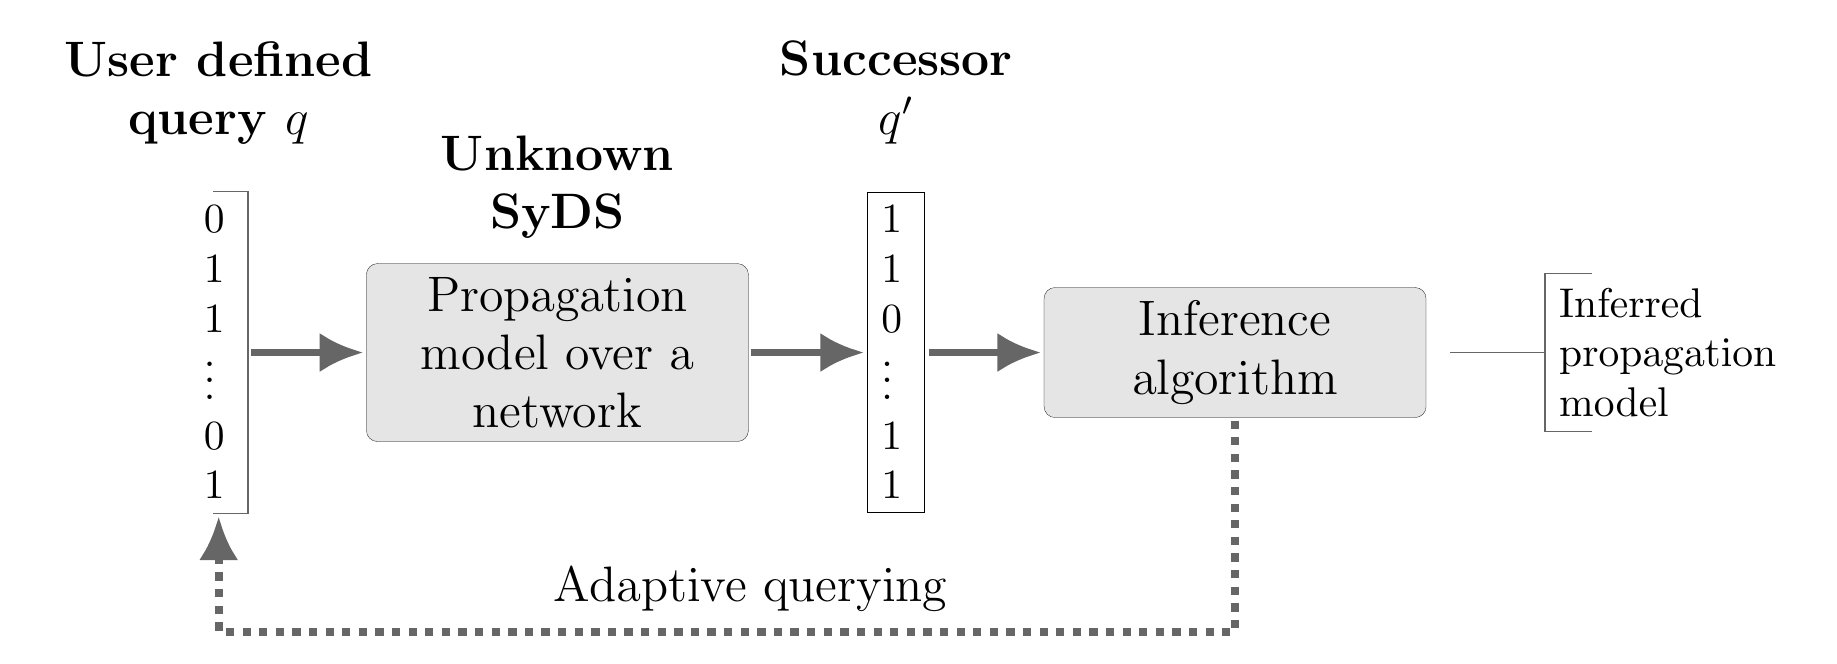
\begin{tikzpicture}
[scale=2,node distance=.5cm, transform shape,
    vertex/.style={shape=circle,fill,inner sep=.7mm},
myblock/.style={draw=none,fill=none,scale=1.5,inner sep=0pt},
every fit/.style={fill=black!10,ellipse,draw=black!20},
myellipse/.style={fill=black!20,draw=none},
edge/.style={black!60,line width=1mm},
edgearr/.style={edge,-{Latex[width=5mm]},shorten >= 1pt,shorten <= 1pt},
block/.style={draw=black,ultra thin,rounded corners,fill=black!10}]
%%%%%%%%%%
%% framework
\begin{scope}[shift={(2.5,-1)},scale=.75,transform shape,node distance=1cm]
%%
\node[] (q) {\parbox{.25cm}{0\\1\\1\\$\vdots$\\0\\1}};
%%
\node [above of=q,shift={(0,1.2)},font=\large] {\parnode{\bf User defined
query~$q$}};
\node (gds) [block,right=of q,font=\large] {\parnode{Propagation model over a
network}};
\node [above of=gds,shift={(0,.4)},font=\large] {\parnode{\bf Unknown SyDS}};
\draw[edgearr] (q.east) -- (gds);
\draw [black!60,line width=.2mm] (q.east) |- (q.north east) -- +(-.3,0);
\draw [black!60,line width=.2mm] (q.east) |- (q.south east) -- +(-.3,0);
\node[right=of gds,draw] (qp) {\parbox{.25cm}{1\\1\\0\\$\vdots$\\1\\1}};
%%
\node [above of=qp,shift={(0,1.2)},font=\large] {\parbox{2cm}{\centering\bf Successor 
$q'$}};
\node (inf) [block,right=of qp,font=\large] {\parnode{Inference algorithm}};
\node (result) [right=of inf] {\parbox{2cm}{Inferred propagation model}};
%%
\draw[edgearr] (gds.east) -- (qp);
\draw[edgearr] (qp) -- (inf);
\draw [edge,line width=.2mm] ($(inf.east)+(.2,0)$) -- (result) -|
(result.north west) -- +(.4,0);
\draw [edge,line width=.2mm] (result) -| (result.south west) -- +(.4,0);
\draw [edgearr,dashed] (inf) |- ($(q.south)+(0,-1)$) -- (q);
\node [shift={(4.5,-2)}, font=\large]{Adaptive querying};
\end{scope}
%%
\end{tikzpicture}
\end{document}
